\documentclass[hyperref={pdfpagelabels=false},compress]{beamer}
\usepackage{lmodern}
\usepackage[utf8]{inputenc}
\usepackage{amssymb}
\usepackage{amsmath}
\graphicspath{{pictures/}}
\usetheme{Singapore}
\usepackage{siunitx}
\usepackage[european]{circuitikz}

\title{Abschlusspräsentation Forschungspraxis: Validierung von Holomorphic Embedding Load Flow}
\author[Schmidt]{Benedikt~Schmidt~(benediktibk@aon.at)}
\institute{Technische Universität München, Germany}
\date{September ??, 2014}

\begin{document}
\begin{frame}
	\titlepage
\end{frame}

\begin{frame}
	\frametitle{Gliederung}
	\tableofcontents
\end{frame}

\section{Holomorphic Embedding Load Flow (HELM)}
\begin{frame}
	\frametitle{Lastflussproblem}
	\begin{figure}
		\centering
		\begin{circuitikz}[scale=0.6, transform shape]
	\draw (0, 0) node[below] {$S_1$} to [R=$Y_{12}$,*-*] (3, 0) node[below] {$S_2$};
	\draw (0, 0) to [R=$Y_{13}$,*-*] (0, 3) node[left] {$S_3$};
	\draw (3, 0) to [R=$Y_{24}$,*-*] (6, 1.5) node[right] {$|U_4|$, $P_4$};
	\draw (3, 3) to [R=$Y_{54}$,*-*] (6, 1.5);
	\draw (0, 3) to [R=$Y_{35}$,*-*] (3, 3) node[below] {$S_5$};
	\draw (3, 3) to [R=$Y_{56}$,*-*] (3, 6) node[left] {$U_6$};
\end{circuitikz} 

	\end{figure}	
	\begin{equation*}
		\sum_j Y_{ij} U_{j} = I_j + \frac{S_j^\star}{U_j^\star}
	\end{equation*}
\end{frame}

\begin{frame}
	\frametitle{Embedding}
	\begin{equation*}
		\sum_j Y_{ij} U_{j}(s) = s I_j + \frac{s S_j^\star}{U_j^\star} + (1 - s) \sum_j Y_{ij}
	\end{equation*}
	
	\begin{equation*}
		U_i \rightarrow U_i(s)
	\end{equation*}
\end{frame}

\begin{frame}
	\frametitle{Berechnung}
	\begin{enumerate}
		\item Einsetzen der Laurent-Reihe
			\begin{equation*}
				U_i(s) = \sum_{n = 0}^\infty c_{i,n} s^n
			\end{equation*}
		\item Berechnung der Koeffizienten durch Entwicklung an $s = 0$
		\item Auswertung an $s = 1$ über analytische Fortsetzung, z.B.: Epsilon Wynn
	\end{enumerate}
\end{frame}

\section{Implementierung}

\begin{frame}
	\frametitle{Allgemein}
	\begin{itemize}
		\item Entwickelt in C++ und C\#
		\item Netze in SQL-Datenbank (Einspeisungen, Transformatoren, Lasten, ...)
		\item GUI um Netze zu bearbeiten
		\item Berechnung der Knotenspannungen
	\end{itemize}
\end{frame}

\begin{frame}
	\frametitle{Verfahren}
	Implementierte Verfahren
	\begin{itemize}
		\item Knotenpunktpotentialverfahren
		\item Stromiteration
		\item Newton-Raphson
		\item Fast-decoupled-load-flow (FDLF)
		\item HELM, 64 Bit Genauigkeit
		\item HELM, beliebige Genauigkeit
	\end{itemize}
\end{frame}

\begin{frame}
	\frametitle{Datenbank}	
	\begin{figure}
		\centering
		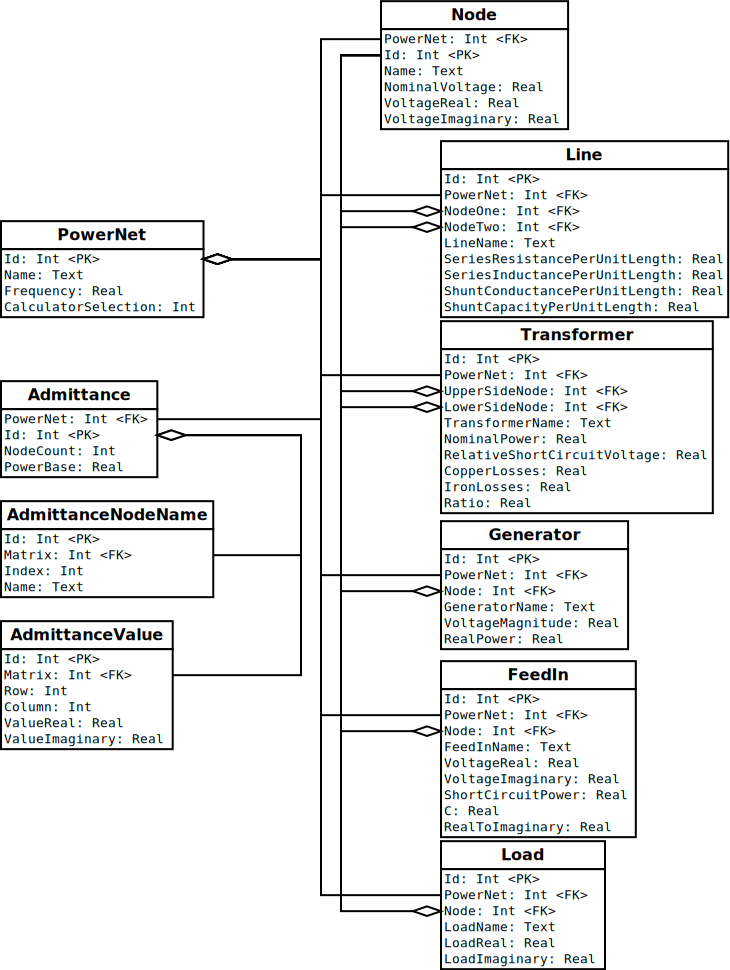
\includegraphics[scale=0.15]{pictures/database_schema}
	\end{figure}
\end{frame}

\section{Ergebnisse}

\begin{frame}
	\frametitle{CalculationComparison}
\end{frame}

\begin{frame}
	\frametitle{Konvergenzverhalten}	
	\begin{figure}
		\centering
		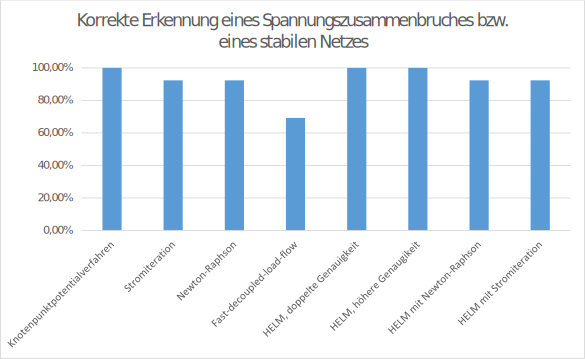
\includegraphics[scale=0.6]{pictures/convergence}
	\end{figure}
\end{frame}

\begin{frame}
	\frametitle{Genauigkeit}
	\begin{figure}
		\centering
		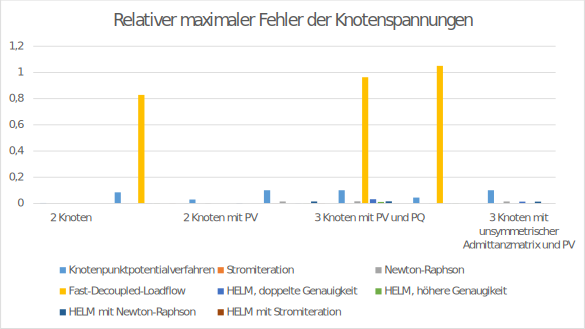
\includegraphics[scale=0.6]{pictures/precision_1}
	\end{figure}
\end{frame}

\begin{frame}
	\frametitle{Genauigkeit}	
	\begin{figure}
		\centering
		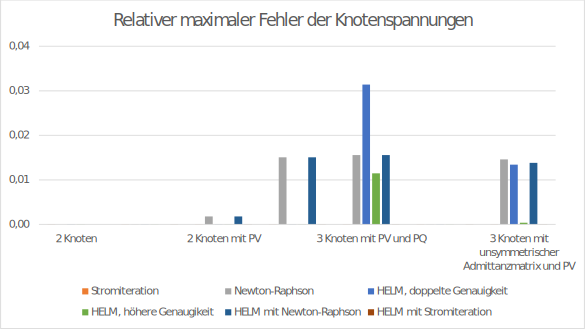
\includegraphics[scale=0.6]{pictures/precision_2}
	\end{figure}
\end{frame}

\begin{frame}
	\frametitle{Berechnungsdauer}	
	\begin{figure}
		\centering
		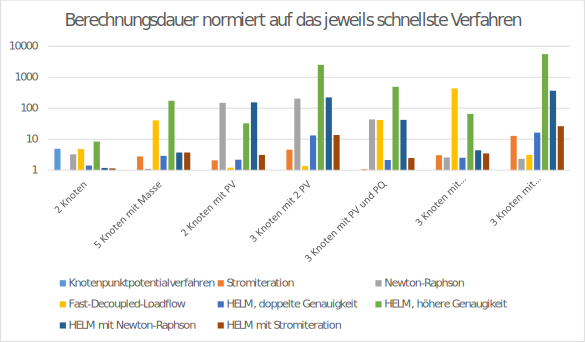
\includegraphics[scale=0.6]{pictures/duration_mean}
	\end{figure}
\end{frame}

\begin{frame}
	\frametitle{Ermittlung der Konvergenzgrenze}	
	\begin{figure}
		\centering
		\begin{circuitikz}	
	\draw (0, 0) node[above] {$U_1$} to [R=$Z$,o-o] (4, 0) node[above] {$U_2$};
	\draw[-stealth] (4, 0) --++ (0,-1);
	\draw (4.5, -1) node {$P$};
\end{circuitikz} 

	\end{figure}
	\begin{itemize}
		\item Bisektion zur Ermittlung der maximalen Last, für den die Verfahren noch konvergieren
		\item Maximum liegt bei $P = \SI{0.25}{\watt}$
	\end{itemize}
\end{frame}

\begin{frame}
	\frametitle{Konvergenzgrenze}
	\begin{figure}
		\centering
		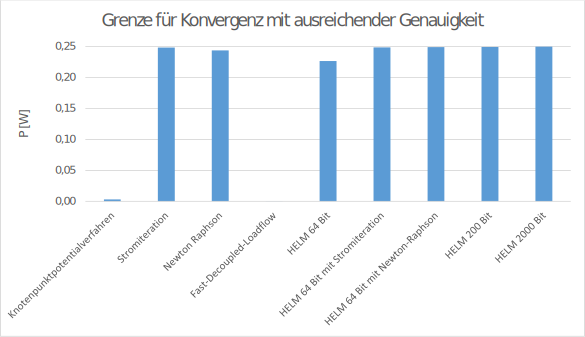
\includegraphics[scale=0.6]{pictures/convergence_border_1}
	\end{figure}
\end{frame}

\begin{frame}
	\frametitle{Konvergenzgrenze}
	\begin{figure}
		\centering
		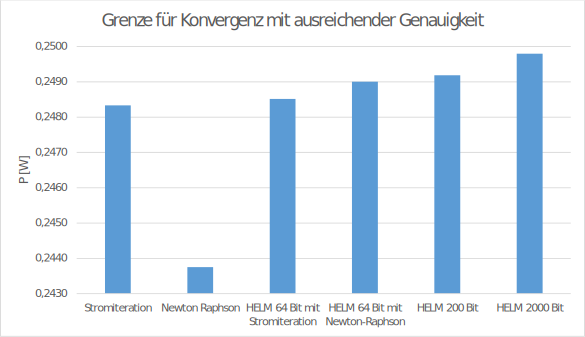
\includegraphics[scale=0.6]{pictures/convergence_border_2}
	\end{figure}
\end{frame}

\section{Fazit}
\begin{frame}
	\frametitle{HELM - Fazit}
	\begin{itemize}
		\item[$-$] Deutlich langsamer als iterative Verfahren
		\item[$+$] Besseres Konvergenzverhalten in der Nähe des Spannungszusammenbruchs 
	\end{itemize}
	
	\begin{itemize}
		\item Theoretisch optimal, praktisch sehr rechenzeitaufwändig
		\item Alternative zu iterative Verfahren
		\item Kombination mit iterativen Verfahren bietet sich an
	\end{itemize}
\end{frame}

\end{document}
